% BAB III Metode Penelitian. Sub-bab baku: Pedoman Tabel 52; isi: Subbab 10.5.
\chapter{Metode Penelitian}
\label{bab:metode}

\panduan{BAB III menunjukkan bahwa penelitian dapat dilaksanakan dan
hasilnya dapat diaudit. Setiap keputusan metodologis ditulis dengan
justifikasi, bukan hanya disebut namanya. Ujiannya sederhana: apakah orang
lain dapat mengulang penelitian ini hanya dengan membaca naskah
(Subbab 10.5). Pada naskah proposal, bab ini ditutup dengan Gantt Chart
riset 16 minggu (Subbab 10.5.4). Pada naskah akhir, ubah kalimat rencana
menjadi laporan pelaksanaan (Subbab 11.2.1).}

\section{Desain Penelitian}
\label{sec:desain}

\panduan{Kerangka umum sama untuk ketiga klaster, tetapi isi desain
berbeda (Subbab 10.5.1, Tabel 47). PL1: eksperimen terkontrol dengan
baseline, studi ablasi, protokol partisi bebas kebocoran data, dan skema
uji signifikansi yang ditetapkan sebelum eksperimen. PL2: siklus
user-centered design dari empati sampai uji kegunaan. PL3: asesmen tata
kelola, audit berbasis bukti, atau implementasi modul dengan skenario UAT.}

Contoh rujukan desain: penelitian yang menghasilkan artefak dapat
mengikuti metodologi design science yang memisahkan siklus perancangan
dan siklus investigasi \cite{wieringa2014design}. Tahapan penelitian
diringkas pada Gambar~\ref{fig:alur-penelitian}.

\begin{figure}[htbp]
  \centering
  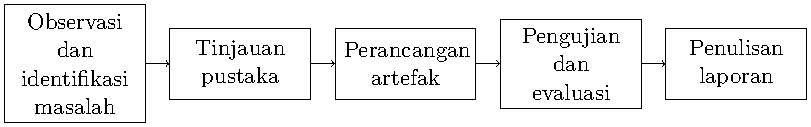
\includegraphics{figures/alur-penelitian.pdf}
  \caption{Contoh alur tahapan penelitian}
  \label{fig:alur-penelitian}
  \sumber{olahan penulis}
\end{figure}

\section{Data, Populasi, atau Sampel}
\label{sec:data}

\panduan{Jawab tiga pertanyaan desain sampling dalam urutan berikut
(Subbab 10.5.2). (1) Populasi sasaran: batas wilayah, periode, serta
kriteria inklusi dan eksklusi. (2) Teknik pemilihan unit beserta
justifikasi tertulis. (3) Jumlah unit yang dihitung dengan formula yang
jejaknya dapat ditelusuri, bukan berdasarkan kebiasaan. Pada PL2, jumlah
responden uji kegunaan minimal 15 orang. Jumlah di bawah batas itu merupakan
temuan kritis (Buku Panduan Dosen, Lembar Audit PL2).}

Tuliskan definisi populasi, teknik sampling, dan perhitungan jumlah
sampel di sini.

\section{Instrumen dan Perangkat}
\label{sec:instrumen}

\panduan{Muat desain instrumen beserta rencana uji validitas dan
reliabilitas dengan ambang keputusan yang dicantumkan sejak proposal
(Subbab 10.5.2). Nama pustaka perangkat lunak beserta versinya hanya
disebut pada bab ini sebagai alat bantu, sedangkan parameter teknisnya diformalkan
secara matematis (Subbab 11.3.1).}

Contoh penyebutan rujukan perangkat: aplikasi yang dievaluasi memakai
gaya arsitektur berbasis sumber daya yang diakses melalui protokol HTTP
\cite{fielding2000rest}. Sebutkan nama dan versi setiap pustaka
perangkat lunak yang dipakai.

\section{Tahapan Pengembangan atau Eksperimen}
\label{sec:tahapan}

\panduan{Prosedur komputasi yang panjang ditulis sebagai algoritma
berlangkah bernomor dengan simbol, bukan nama fungsi pustaka
(Subbab 11.3.3 butir 1). Kode sumber lengkap ditempatkan di lampiran atau
repositori dan dirujuk dari teks (Subbab 11.3.1).}

Prosedur perhitungan skor kegunaan setiap responden dirumuskan pada
Algoritma~\ref{alg:sus}. Implementasinya dimuat pada
Lampiran~\ref{lamp:kode}.

\begin{algorithm}[htbp]
  \caption{Contoh perhitungan skor SUS per responden}
  \label{alg:sus}
  \begin{algorithmic}[1]
    \Require jawaban $x_{i1},\dots,x_{i10} \in \{1,\dots,5\}$ responden ke-$i$
    \Ensure skor $S_i \in [0,100]$
    \State $T \gets 0$
    \For{$j \gets 1$ \textbf{sampai} $10$}
      \If{$j$ ganjil}
        \State $T \gets T + (x_{ij} - 1)$
      \Else
        \State $T \gets T + (5 - x_{ij})$
      \EndIf
    \EndFor
    \State \Return $S_i = 2,5\,T$
  \end{algorithmic}
\end{algorithm}

\section{Metrik dan Uji Statistik}
\label{sec:metrik}

\panduan{Setiap metrik ditulis sebagai persamaan bernomor. Simbol
didefinisikan pada kalimat yang mendahului atau menyertai persamaan,
dengan arti, himpunan nilai, dan satuan bila ada. Satu simbol hanya satu
arti di seluruh naskah, dan bilangan desimal ditulis dengan koma
(Subbab 11.4). Cantumkan sumber formula yang dikutip.}

Skor SUS responden ke-$i$ dihitung dengan Persamaan~\eqref{eq:sus}
\cite{brooke1996sus}, dengan $x_{ij}$ skor butir ke-$j$ pada skala 1
sampai 5.
\begin{equation}
  S_i = 2,5 \left( \sum_{j \in \{1,3,5,7,9\}} (x_{ij} - 1)
        + \sum_{j \in \{2,4,6,8,10\}} (5 - x_{ij}) \right)
  \label{eq:sus}
\end{equation}
Rerata skor dari $n$ responden dihitung dengan Persamaan~\eqref{eq:rerata}.
\begin{equation}
  \bar{S} = \frac{1}{n} \sum_{i=1}^{n} S_i
  \label{eq:rerata}
\end{equation}

\section{Etika dan Keamanan Data}
\label{sec:etika}

\panduan{Jelaskan perizinan, persetujuan responden (informed consent),
anonimisasi, dan penyimpanan data sesuai Undang-Undang Pelindungan Data
Pribadi (Pedoman Subbab 2.3). Data mitra yang belum dianonimkan tidak
masuk repositori mana pun (Subbab 14.5). Pengambilan data tanpa izin dan
informed consent merupakan temuan kritis (Subbab 13.7.2).}

Contoh rujukan regulasi dan standar: pengolahan data pribadi responden
mengikuti ketentuan undang-undang yang berlaku \cite{uupdp2022}, dan
pengamanan berkas data mengacu pada persyaratan sistem manajemen keamanan
informasi \cite{iso27001}.
